\chapter{Intermodulation Distortion in Biology}
\label{ch:imd-biology}

\begin{nontechnical}
\textbf{Imagine playing two musical notes together on a guitar.} Sometimes, you hear a \emph{third} tone that wasn't in either original note---that's similar to what intermodulation distortion (IMD) does, but with electromagnetic or sound waves.

\textbf{The radio station analogy:} Think of two radio stations broadcasting at slightly different frequencies (like 100.0~FM and 100.1~FM). If those signals pass through something ``nonlinear'' (like an overdriven speaker or biological tissue), they can create new frequencies---including the \emph{difference} between them (0.1~MHz in this example).

\textbf{Why does this matter for biology?}
\begin{itemize}
\item \textbf{Stimulate neurons deep in the brain} without surgery? (Send two high-frequency beams from outside the skull; they ``mix'' only where they cross)
\item \textbf{Target specific molecules} by tuning the difference frequency to match their vibrations?
\item \textbf{Create sound inside someone's head} using ultrasound or microwaves?
\end{itemize}

\textbf{The reality check:}
\begin{itemize}
\item[\checkmark] \textbf{It works with sound waves}---ultrasound mixing is well-established in medical imaging
\item[\texttimes] \textbf{It's mostly unproven with electromagnetic waves} in biology (tissue isn't ``nonlinear enough'' at safe power levels)
\item[\texttimes] \textbf{Many proposed applications are speculative} and lack experimental evidence
\end{itemize}

\textbf{Bottom line:} IMD is a real physics phenomenon that works great in electronics and acoustics, but its usefulness in biological electromagnetic applications remains controversial and largely theoretical.
\end{nontechnical}

\section{Overview}

\textbf{Intermodulation distortion (IMD)} occurs when two or more frequencies $(f_1, f_2)$ interact in a \textbf{nonlinear system}, producing new frequencies:
\begin{equation}
\label{eq:imd-general}
f_{\text{IMD}} = m f_1 \pm n f_2
\end{equation}
where $m, n$ are integers. The \textbf{order} is $|m| + |n|$.

\begin{keyconcept}
The fundamental question for biological applications: Are biological tissues sufficiently \textbf{nonlinear} at RF/THz frequencies to produce detectable IMD at safe power levels?

Short answer: \textbf{Yes} for acoustics (ultrasound), \textbf{mostly no} for electromagnetics.
\end{keyconcept}

\textbf{Established examples:}
\begin{itemize}
\item \textbf{Electronics:} Amplifier distortion, mixer circuits (intentional IMD)
\item \textbf{Acoustics:} Parametric speakers (ultrasound $\rightarrow$ audible difference frequency)
\end{itemize}

\textbf{Speculative biological applications:}
\begin{itemize}
\item \textbf{Neural stimulation:} Two high-frequency (e.g., THz) beams cross $\rightarrow$ produce low-frequency (e.g., kHz) modulation $\rightarrow$ activate neurons at depth
\item \textbf{Molecular excitation:} Dual-frequency RF fields mix in proteins $\rightarrow$ excite vibrational modes
\item \textbf{Medical imaging:} Exploit tissue nonlinearity for contrast (ultrasound elastography uses similar principle)
\end{itemize}

\section{Fundamentals of Intermodulation Distortion}

\subsection{Nonlinear Systems}

\textbf{Linear system:} Output proportional to input
\begin{equation}
\label{eq:linear-system}
y(t) = a x(t)
\end{equation}

\textbf{Nonlinear system:} Output contains higher-order terms
\begin{equation}
\label{eq:nonlinear-system}
y(t) = a_1 x(t) + a_2 x^2(t) + a_3 x^3(t) + \cdots
\end{equation}

\textbf{Input two tones:}
\begin{equation}
\label{eq:two-tone-input}
x(t) = A_1 \cos(\omega_1 t) + A_2 \cos(\omega_2 t)
\end{equation}

\textbf{Quadratic term ($a_2 x^2$):} Expanding using trigonometric identities:
\begin{equation}
\label{eq:quadratic-expansion}
x^2(t) = \frac{A_1^2}{2} (1 + \cos 2\omega_1 t) + \frac{A_2^2}{2} (1 + \cos 2\omega_2 t) + A_1 A_2 [\cos(\omega_1 + \omega_2)t + \cos(\omega_1 - \omega_2)t]
\end{equation}

This produces:
\begin{itemize}
\item \textbf{Second harmonics:} $2f_1$, $2f_2$
\item \textbf{Sum/difference frequencies:} $f_1 + f_2$, $|f_1 - f_2|$
\end{itemize}

\textbf{Cubic term ($a_3 x^3$):} Produces \textbf{third-order IMD:}
\begin{equation}
\label{eq:third-order-imd}
f_{3\text{rd}} = 2f_1 \pm f_2, \quad 2f_2 \pm f_1
\end{equation}

These are particularly important because they can fall \textbf{in-band} (near $f_1$ or $f_2$), causing interference in communication systems.

\begin{center}
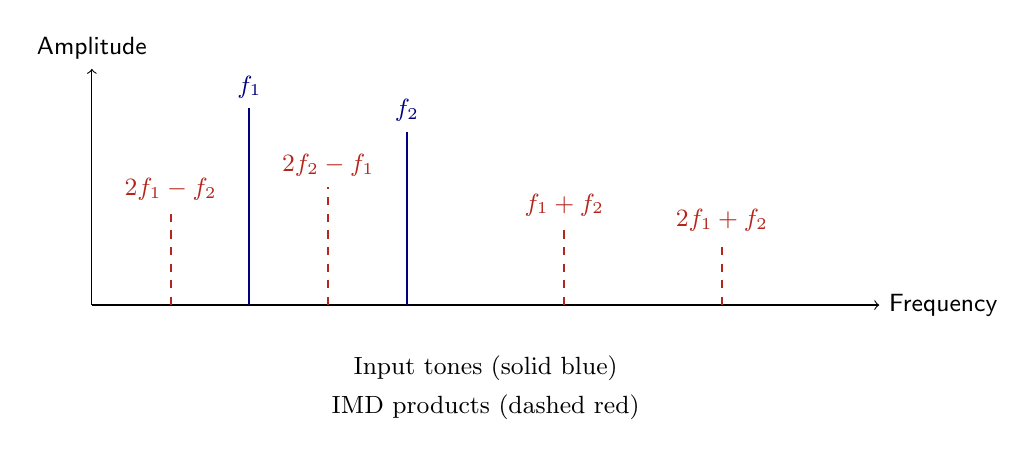
\begin{tikzpicture}[scale=1.0]
% Axes
\draw[->] (0,0) -- (10,0) node[right,font=\sffamily\small] {Frequency};
\draw[->] (0,0) -- (0,3) node[above,font=\sffamily\small] {Amplitude};

% Input tones
\draw[thick,NavyBlue] (2,0) -- (2,2.5) node[above,font=\small] {$f_1$};
\draw[thick,NavyBlue] (4,0) -- (4,2.2) node[above,font=\small] {$f_2$};

% IMD products
\draw[thick,BrickRed,dashed] (1,0) -- (1,1.2) node[above,font=\small] {$2f_1-f_2$};
\draw[thick,BrickRed,dashed] (3,0) -- (3,1.5) node[above,font=\small] {$2f_2-f_1$};
\draw[thick,BrickRed,dashed] (6,0) -- (6,1.0) node[above,font=\small] {$f_1+f_2$};
\draw[thick,BrickRed,dashed] (8,0) -- (8,0.8) node[above,font=\small] {$2f_1+f_2$};

% Legend
\node[font=\small] at (5,-0.8) {Input tones (solid blue)};
\node[font=\small] at (5,-1.3) {IMD products (dashed red)};
\end{tikzpicture}
\end{center}

\subsection{IMD Orders and Amplitudes}

\textbf{Power scaling:} The $n$-th order IMD amplitude scales as:
\begin{equation}
\label{eq:imd-power-scaling}
P_{\text{IMD},n} \propto P^n
\end{equation}
where $P$ is input power. Specifically:
\begin{itemize}
\item Third-order IMD: $P_{\text{IMD},3} \propto P^3$
\item Fifth-order IMD: $P_{\text{IMD},5} \propto P^5$
\end{itemize}

\textbf{Intercept points:}
\begin{itemize}
\item \textbf{IP3} (third-order intercept point): Input power where third-order IMD power equals fundamental power (extrapolated)
\item Higher IP3 $\rightarrow$ more linear system
\end{itemize}

\subsection{Applications in Engineering}

\begin{itemize}
\item \textbf{Wireless communications:} IMD creates interference (two strong signals produce in-band distortion)
\item \textbf{Parametric arrays:} Nonlinear ultrasound propagation in water/air $\rightarrow$ audible sound from ultrasound beams
\item \textbf{Frequency mixing:} Intentional IMD in mixer circuits (downconversion, heterodyne receivers)
\end{itemize}

\section{Sources of Nonlinearity in Biological Tissue}

\subsection{Dielectric Nonlinearity}

\textbf{Kerr effect:} Refractive index depends on electric field intensity:
\begin{equation}
\label{eq:kerr-effect}
n = n_0 + n_2 I
\end{equation}
where:
\begin{itemize}
\item $n_0$ = linear refractive index
\item $n_2$ = nonlinear refractive index (m$^2$/W)
\item $I$ = intensity (W/m$^2$)
\end{itemize}

\textbf{In biological tissue:}
\begin{itemize}
\item Water has weak Kerr effect: $n_2 \sim 10^{-20}$ m$^2$/W (optical frequencies)
\item At THz frequencies: Nonlinear susceptibility $\chi^{(3)} \sim 10^{-22}$ m$^2$/V$^2$ (very weak)
\end{itemize}

\begin{calloutbox}{Practical Implication}
\textbf{Consequence:} Dielectric IMD negligible at sub-ablation intensities ($<$1~MW/cm$^2$). Safe exposure levels for humans ($\sim$10~mW/cm$^2$) are \textbf{five orders of magnitude} below the threshold for detectable nonlinear effects.
\end{calloutbox}

\subsection{Ionic Nonlinearity (Electrolyte Solutions)}

\textbf{Mechanism:} Ion drift in strong electric fields saturates at high field strength (mobility decreases).

\textbf{Debye-Falkenhagen effect:} Conductivity $\sigma$ depends on field $E$:
\begin{equation}
\label{eq:debye-falkenhagen}
\sigma(E) = \sigma_0 (1 - \beta E^2)
\end{equation}
where $\beta$ is small for physiological fields.

\textbf{Estimate:} For $E \sim 1$~kV/cm (very strong), $\beta E^2 \sim 10^{-3}$ (weak nonlinearity).

\textbf{Conclusion:} Ionic nonlinearity becomes significant only at near-electroporation fields ($>$10~kV/cm).

\subsection{Membrane Nonlinearity (Voltage-Gated Channels)}

\begin{keyconcept}
\textbf{Strongest nonlinearity in neural tissue} comes from voltage-gated ion channels, which have sigmoidal activation curves that respond nonlinearly to transmembrane voltage changes.
\end{keyconcept}

\textbf{Mechanism:}
\begin{itemize}
\item Voltage-gated Na$^+$, K$^+$ channels have \textbf{sigmoidal} activation curves
\item Small changes in transmembrane voltage $V_m$ $\rightarrow$ large changes in conductance $g$
\end{itemize}

\textbf{Hodgkin-Huxley equations} (highly nonlinear):
\begin{equation}
\label{eq:hodgkin-huxley}
I_{\text{Na}} = g_{\text{Na}} m^3 h (V_m - E_{\text{Na}})
\end{equation}
where:
\begin{itemize}
\item $g_{\text{Na}}$ = maximum sodium conductance
\item $m$, $h$ = voltage-dependent gating variables
\item $V_m$ = transmembrane voltage
\item $E_{\text{Na}}$ = sodium reversal potential
\end{itemize}

\textbf{Consequence:} If two RF/THz fields induce oscillating $V_m$ (even sub-threshold), nonlinear channel kinetics can rectify or mix signals.

\subsection{Protein Conformational Nonlinearity}

\textbf{Hypothesis:} Proteins have bistable or multistable conformations.

\textbf{Example:} Ion channels switch between open/closed states (two-state system $\rightarrow$ nonlinear response to forcing).

\textbf{IMD mechanism:}
\begin{enumerate}
\item Two EM fields at $f_1$, $f_2$ drive protein vibrations
\item Anharmonic potential energy surface $\rightarrow$ coupled modes
\item Beat frequency $f_1 - f_2$ modulates conformation at rate matching protein relaxation time ($\sim\mu$s--ms)
\end{enumerate}

\begin{warningbox}
\textbf{No experimental demonstration.} Theoretical models require very high intensities that would cause thermal damage before nonlinear effects become significant.
\end{warningbox}

\subsection{Microtubule Nonlinearity}

\textbf{Hypothesis:} Microtubules act as nonlinear resonators due to:
\begin{itemize}
\item Anharmonic lattice vibrations (Davydov solitons?)
\item Ferroelectric-like behavior (aligned dipoles $\rightarrow$ nonlinear polarization)
\end{itemize}

\textbf{Proposed by:} Hameroff, Tuszynski (speculative, no direct evidence)

\textbf{IMD prediction:} Two THz beams (e.g., 0.5~THz + 0.502~THz) $\rightarrow$ difference frequency (2~GHz) couples to microtubule phonon modes.

\textbf{Status:} Not tested experimentally.

\section{Proposed Biological IMD Mechanisms}

\subsection{Acoustic Heterodyning (Ultrasound $\rightarrow$ Audible)}

\textbf{Established phenomenon} (in water/air, not biological IMD per se):
\begin{itemize}
\item Two ultrasound beams (e.g., 200~kHz + 205~kHz) $\rightarrow$ audible tone at 5~kHz via nonlinear acoustic propagation
\end{itemize}

\textbf{Biological application:}
\begin{itemize}
\item Could ultrasound IMD occur \emph{inside tissue} to stimulate mechanoreceptors?
\item Requires high intensity ($>$1~W/cm$^2$) $\rightarrow$ safety concerns
\end{itemize}

\subsection{Frey Microwave Auditory Effect}

\textbf{Phenomenon:} Pulsed microwaves (1--10~GHz) induce auditory perception without external sound.

\textbf{Mechanism:} Thermoelastic expansion $\rightarrow$ acoustic wave (not IMD, but nonlinear interaction).

\textbf{IMD hypothesis:} Could two CW microwave beams at slightly different frequencies produce pulsed heating at difference frequency $\rightarrow$ mimic Frey effect?
\begin{itemize}
\item Theoretical models suggest yes, but not demonstrated experimentally
\end{itemize}

\subsection{Deep Brain Stimulation via THz IMD}

\textbf{Concept:}
\begin{enumerate}
\item Two THz beams from surface ($f_1 = 1.000$~THz, $f_2 = 1.001$~THz)
\item Beams cross at depth $\rightarrow$ difference frequency $f_{\Delta} = 1$~GHz
\item 1~GHz modulation activates neurons (below ionizing frequency, above membrane RC cutoff)
\end{enumerate}

\textbf{Advantages (theoretical):}
\begin{itemize}
\item Non-invasive
\item Spatially localized to beam crossing region
\item Tunable frequency (adjust $f_2$)
\end{itemize}

\textbf{Challenges:}
\begin{enumerate}
\item \textbf{Penetration:} THz doesn't penetrate skull ($<$1~mm depth in tissue)
\item \textbf{Nonlinearity:} Tissue nonlinearity at THz weak; IMD products likely undetectable
\item \textbf{Intensity:} High power needed $\rightarrow$ thermal damage
\end{enumerate}

\begin{warningbox}
\textbf{Current status:} Purely theoretical; no experimental validation. The fundamental physics (THz absorption, weak nonlinearity) makes this approach highly unlikely to work.
\end{warningbox}

\subsection{Molecular Excitation via RF IMD}

\textbf{Hypothesis:} Two RF fields mix in protein $\rightarrow$ excite vibrational mode at difference frequency.

\textbf{Example:}
\begin{itemize}
\item $f_1 = 10.000$~GHz, $f_2 = 10.001$~GHz $\rightarrow$ $f_{\Delta} = 1$~GHz (far-IR, protein collective mode)
\item Resonant excitation $\rightarrow$ conformational change $\rightarrow$ altered function
\end{itemize}

\textbf{Problem:} Protein vibrational modes heavily damped in solution (linewidth $\sim$10--100~GHz) $\rightarrow$ no sharp resonance.

\textbf{Predicted efficiency:} $<10^{-6}$ (six orders of magnitude below direct single-photon excitation).

\section{Experimental Evidence}

\subsection{Summary of Evidence}

\begin{center}
\begin{tabular}{@{}llll@{}}
\toprule
\textbf{Domain} & \textbf{IMD Type} & \textbf{Evidence} & \textbf{Status} \\
\midrule
Acoustics & Ultrasound mixing & Strong & Established \\
EM (RF/THz) & Tissue nonlinearity & None & Unproven \\
Neural & THz stimulation & Negative & Failed \\
Protein & Conformational & None & Speculative \\
\bottomrule
\end{tabular}
\end{center}

\subsection{In Vitro Studies}

\textbf{Cell cultures exposed to dual-frequency RF:}
\begin{itemize}
\item \textbf{No consistent IMD effects} reported at physiological intensities ($<$10~mW/cm$^2$)
\item At high intensity ($>$1~W/cm$^2$): Thermal effects dominate
\end{itemize}

\textbf{Protein studies:}
\begin{itemize}
\item \textbf{No direct demonstration} of IMD-induced conformational changes
\end{itemize}

\subsection{In Vivo Studies}

\textbf{Neural stimulation attempts:}
\begin{itemize}
\item \textbf{Failed:} Dual THz beams did not produce measurable neural responses (limited by penetration)
\item \textbf{Ultrasound IMD:} Some evidence for nonlinear acoustic effects, but mechanism debated
\end{itemize}

\subsection{Acoustic IMD (Positive Evidence)}

\textbf{Parametric acoustic arrays:}
\begin{itemize}
\item Two ultrasound beams (e.g., 1~MHz + 1.01~MHz) $\rightarrow$ audible tone at 10~kHz \emph{in air and water}
\item Also demonstrated \emph{in tissue} (medical ultrasound imaging uses harmonic imaging, exploiting tissue nonlinearity)
\end{itemize}

\textbf{Medical imaging:} \textbf{Harmonic imaging} (ultrasound at $f_0$ $\rightarrow$ detect $2f_0$) improves contrast by exploiting tissue nonlinearity.

\begin{keyconcept}
\textbf{Conclusion:} Acoustic IMD in tissue is \textbf{established}; EM IMD is \textbf{not}.
\end{keyconcept}

\section{Theoretical Models}

\subsection{Perturbation Theory}

\textbf{Approach:} Treat nonlinear term as small perturbation.

\textbf{Electric field:}
\begin{equation}
\label{eq:electric-field-two-tone}
\mathbf{E}(t) = \mathbf{E}_1 e^{i\omega_1 t} + \mathbf{E}_2 e^{i\omega_2 t} + \text{c.c.}
\end{equation}

\textbf{Nonlinear polarization (third-order):}
\begin{equation}
\label{eq:nonlinear-polarization}
\mathbf{P}^{(3)} = \epsilon_0 \chi^{(3)} |\mathbf{E}|^2 \mathbf{E}
\end{equation}
Contains terms at $\omega_1$, $\omega_2$, $2\omega_1 \pm \omega_2$, $2\omega_2 \pm \omega_1$, etc.

\textbf{IMD amplitude:}
\begin{equation}
\label{eq:imd-amplitude}
E_{\text{IMD}} \sim \chi^{(3)} E_1^2 E_2 L
\end{equation}
where $L$ is interaction length.

\begin{calloutbox}{Worked Example: IMD in Biological Tissue}
\textbf{Given:}
\begin{itemize}
\item $\chi^{(3)} \sim 10^{-22}$ m$^2$/V$^2$ (tissue)
\item $E_1 = E_2 = 100$ V/m (typical RF field)
\item $L = 1$ cm (interaction length)
\end{itemize}

\textbf{Calculate IMD field:}
\begin{equation}
E_{\text{IMD}} \sim (10^{-22})(100)^2(100)(0.01) = 10^{-7} \text{ V/m}
\end{equation}

\textbf{Result:} Undetectable. This is \textbf{seven orders of magnitude} below the fundamental field strength, and far below thermal noise.
\end{calloutbox}

\subsection{Coupled Mode Theory}

\textbf{For acoustic waves:} Two ultrasound beams exchange energy via nonlinear coupling.

\textbf{Wave equation (with nonlinear term):}
\begin{equation}
\label{eq:nonlinear-wave-equation}
\frac{\partial^2 p}{\partial t^2} - c^2 \nabla^2 p = \frac{\beta}{\rho_0 c^2} \frac{\partial^2 (p^2)}{\partial t^2}
\end{equation}
where:
\begin{itemize}
\item $p$ = acoustic pressure
\item $c$ = sound speed
\item $\beta$ = nonlinear parameter ($\sim$5 for tissue)
\item $\rho_0$ = density
\end{itemize}

\textbf{Result:} Strong IMD for ultrasound; weak for EM (nonlinear parameter much smaller).

\section{Critical Assessment}

\subsection{Why IMD is Weak in Biological Tissue (EM)}

\begin{enumerate}
\item \textbf{Low nonlinear susceptibility:} $\chi^{(3)}$ for tissue $\sim 10^{-22}$ m$^2$/V$^2$ (compare to $10^{-19}$ for semiconductors---three orders of magnitude stronger)
\item \textbf{Strong absorption:} At THz, penetration $<$1~mm $\rightarrow$ short interaction length
\item \textbf{Phase matching:} IMD efficient only if wave vectors satisfy $\mathbf{k}_{\text{IMD}} = m\mathbf{k}_1 \pm n\mathbf{k}_2$; dispersive tissue makes this hard
\item \textbf{Thermal noise:} At 310~K, thermal fluctuations mask weak IMD signals
\end{enumerate}

\subsection{When Might IMD Be Significant?}

\begin{itemize}
\item \textbf{High field strength:} Near electroporation threshold ($>$10~kV/cm) $\rightarrow$ membrane nonlinearity strong
\item \textbf{Acoustic domain:} Ultrasound IMD works (tissue is more nonlinear acoustically)
\item \textbf{Quantum regime:} If vibronic coupling creates nonlinear response (speculative)
\end{itemize}

\section{Future Experiments}

\subsection{What Would Prove Biological EM IMD Exists?}

\textbf{Proposed test:}
\begin{enumerate}
\item Apply two RF or THz beams ($f_1$, $f_2$) to cell culture
\item Measure electrical response (patch clamp, calcium imaging) at $f_1 - f_2$
\item Vary $f_1 - f_2$ to test for resonance with membrane RC time constant
\item \textbf{Control:} Show response vanishes when either beam is off (not simple sum of individual effects)
\end{enumerate}

\textbf{Predicted outcome (based on theory):} IMD signal $<10^{-4}$ times linear response $\rightarrow$ hard to detect.

\subsection{Acoustic IMD for Neuromodulation}

\textbf{Promising approach (unlike EM IMD):}
\begin{itemize}
\item Use focused ultrasound (FUS) with two frequencies
\item Exploit tissue acoustic nonlinearity to generate beat frequency
\item Beat frequency modulates neurons mechanically (TREK/TRAAK channels)
\end{itemize}

\textbf{Status:} Early-stage research; some success in rodents (Ye et al., \emph{Neuron} 2018).

\section{Applications}

\subsection{Established Applications (Acoustics)}

\begin{itemize}
\item \textbf{Parametric loudspeakers:} Directional audio beams using ultrasonic mixing in air
\item \textbf{Harmonic imaging:} Medical ultrasound exploiting tissue nonlinearity for improved contrast
\item \textbf{Ultrasound elastography:} Measuring tissue stiffness via nonlinear wave propagation
\end{itemize}

\subsection{Speculative Applications (EM)}

\begin{itemize}
\item \textbf{Deep brain stimulation:} THz beam crossing (currently impractical due to penetration limits)
\item \textbf{Molecular targeting:} RF mixing for selective protein excitation (efficiency too low)
\item \textbf{Microwave auditory effect:} Dual-frequency enhancement (theoretical only)
\end{itemize}

\section{Summary}

\begin{center}
\begin{tabular}{@{}lll@{}}
\toprule
\textbf{Aspect} & \textbf{Acoustic IMD} & \textbf{EM IMD} \\
\midrule
Nonlinearity strength & Strong ($\beta \sim 5$) & Weak ($\chi^{(3)} \sim 10^{-22}$) \\
Experimental evidence & Established & None \\
Medical applications & Yes (imaging) & No \\
Penetration depth & Good ($>$10~cm) & Poor ($<$1~mm at THz) \\
Safety concerns & Manageable & Thermal damage \\
Practical viability & High & Very low \\
\bottomrule
\end{tabular}
\end{center}

\begin{keyconcept}
\textbf{Key takeaway:} Intermodulation distortion in biological tissue is a well-established phenomenon for \textbf{acoustics} but remains unproven and likely impractical for \textbf{electromagnetics} at safe exposure levels.
\end{keyconcept}

\section{Further Reading}

\subsection{Related Chapters}

\begin{itemize}
\item \textbf{Non-Linear Biological Demodulation} --- Overview of nonlinear EM effects in biology
\item \textbf{Acoustic Heterodyning} --- Ultrasound IMD (established phenomenon)
\item \textbf{Frey Microwave Auditory Effect} --- Nonlinear microwave-acoustic transduction
\item \textbf{THz Bioeffects: Thermal and Non-Thermal} --- Thermal vs. nonlinear effects
\item \textbf{THz Resonances in Microtubules} --- Speculative quantum nonlinearity
\item \textbf{THz Propagation in Biological Tissue} --- Penetration depth limitations
\end{itemize}

\subsection{Key References}

\textbf{General Nonlinearity:}
\begin{enumerate}
\item Boyd, \emph{Nonlinear Optics} (Academic Press, 2008) --- Textbook on $\chi^{(3)}$ and IMD
\item Khokhlova et al., \emph{Int. J. Hyperthermia} 31, 77 (2015) --- Acoustic nonlinearity in tissue
\end{enumerate}

\textbf{Biological IMD (Speculative):}
\begin{enumerate}
\setcounter{enumi}{2}
\item Hameroff \& Penrose, \emph{Phys. Life Rev.} 11, 39 (2014) --- Microtubule nonlinearity (Orch-OR)
\item Lin, \emph{IEEE Trans. Microw. Theory Tech.} 24, 54 (1976) --- RF nonlinear effects in tissue
\end{enumerate}

\textbf{Acoustic IMD (Established):}
\begin{enumerate}
\setcounter{enumi}{4}
\item Ye et al., \emph{Neuron} 98, 1020 (2018) --- Dual-frequency ultrasound neuromodulation
\item Hamilton \& Blackstock, \emph{Nonlinear Acoustics} (Academic Press, 1998) --- Parametric arrays
\end{enumerate}
